% ------------------------------------------------------------------------
% ------------------------------------------------------------------------
% Modelo UFSC para Trabalhos Academicos (tese de doutorado, dissertação de
% mestrado) utilizando a classe abntex2
%
% Autor: Alisson Lopes Furlani
% 	Modificações:
%	- 27/08/2019: Alisson L. Furlani, add 'glossaries' package
%   - 30/10/2019: Alisson L. Furlani, adjusted some spacing errors and changed math fonts
%   - 17/01/2020: Alisson L. Furlani, updated certification page
%   - 07/02/2020: Alisson L. Furlani, fixed table counter bug
%   - 11/03/2020: Alisson L. Furlani, changed greek letters in math and fixed citation style
% ------------------------------------------------------------------------
% ------------------------------------------------------------------------

\documentclass[
	% -- opções da classe memoir --
	12pt,				% tamanho da fonte
	%openright,			% capítulos começam em pág ímpar (insere página vazia caso preciso)
	oneside,			% para impressão no anverso. Oposto a twoside
	a4paper,			% tamanho do papel.
	% -- opções da classe abntex2 --
	chapter=TITLE,		% títulos de capítulos convertidos em letras maiúsculas
	section=TITLE,		% títulos de seções convertidos em letras maiúsculas
	%subsection=TITLE,	% títulos de subseções convertidos em letras maiúsculas
	%subsubsection=TITLE,% títulos de subsubseções convertidos em letras maiúsculas
	% -- opções do pacote babel --
	english,			% idioma adicional para hifenização
	%french,				% idioma adicional para hifenização
	%spanish,			% idioma adicional para hifenização
	brazil				% o último idioma é o principal do documento
	]{abntex2}

\usepackage{setup/ufscthesisA4-alf}
\usepackage[backend=biber]{biblatex}
\addbibresource{aftertext/references.bib} % Seus arquivos de referências


% MEUS PACOTES

\usepackage{booktabs}
\usepackage{graphicx}
\usepackage{enumitem}
\usepackage{csquotes}
% \usepackage[portuguese, linesnumbered]{algorithm2e}
\usepackage{amsthm}
\usepackage{amssymb}
\usepackage{verbatim}
\usepackage{amsmath}
\usepackage{caption}
\usepackage{algorithm}
% trocar label do algorithm para pt-br
\makeatletter
\renewcommand{\ALG@name}{Algoritmo}
\makeatother
\usepackage{tocbibind}
\usepackage{colortbl}
\usepackage{tabularx}
\usepackage[outputdir=build]{minted}


\usepackage{pdflscape}
\usepackage{makecell}%To keep spacing of text in tables
\setcellgapes{4pt}%parameter for the spacing

\usepackage[table,xcdraw]{xcolor}


\newcolumntype{Y}{>{\centering\arraybackslash}X}
\newcolumntype{P}[1]{>{\centering\arraybackslash}p{#1}}
\newcommand{\centered}[1]{\begin{tabular}{l} #1 \end{tabular}}

\theoremstyle{definition}
\newtheorem{definition}{Definição}
\newtheorem{example}{Exemplo}[section]



% SIGON
\usepackage{listings}
\renewcommand{\lstlistingname}{Código}
\usepackage{xcolor}
\lstset{%
    language=Python,
    basicstyle=\small\ttfamily,%
    numbers=left, numberstyle=\tiny, stepnumber=1, numbersep=5pt,%
    aboveskip=3mm,
    belowskip=3mm,
    showstringspaces=false,
    columns=flexible,
        morekeywords={plan, action, sensor, actuator, sense, member},
    basicstyle={\small},
    numberstyle=\tiny\color{gray},
    keywordstyle={[2]\color{blue}},
    keywordstyle={[3]\color{red}},
    keywordstyle={[4]\color{black}},
    otherkeywords={String,async,await,Task,var},
    keywords=[2]{communication, beliefs, desires, intentions, planner},
    keywords=[3]{:},
    keywords=[4]{sensor, actuator},
    commentstyle=\color{ForestGreen},
    stringstyle=\color{red},
    captionpos=b,
    breaklines=true,
    breakatwhitespace=true,
    tabsize=4
}%

% Don't draw red squares over some characters
\AtBeginEnvironment{minted}{%
  \renewcommand{\fcolorbox}[4][]{#4}}


% ---
% Filtering and Mapping Bibliographies
% ---
\DeclareSourcemap{
	\maps[datatype=bibtex]{
		% remove fields that are always useless
		\map{
			\step[fieldset=abstract, null]
			\step[fieldset=pagetotal, null]
		}
		% remove URLs for types that are primarily printed
%		\map{
%			\pernottype{software}
%			\pernottype{online}
%			\pernottype{report}
%			\pernottype{techreport}
%			\pernottype{standard}
%			\pernottype{manual}
%			\pernottype{misc}
%			\step[fieldset=url, null]
%			\step[fieldset=urldate, null]
%		}
		\map{
			\pertype{inproceedings}
			% remove mostly redundant conference information
			\step[fieldset=venue, null]
			\step[fieldset=eventdate, null]
			\step[fieldset=eventtitle, null]
			% do not show ISBN for proceedings
			\step[fieldset=isbn, null]
			% Citavi bug
			\step[fieldset=volume, null]
		}
	}
}
% ---

% ---
% Informações de dados para CAPA e FOLHA DE ROSTO
% ---
% FIXME Substituir 'Nome completo do autor' pelo seu nome.
\autor{Lucas Zacchi de Medeiros}
% FIXME Substituir 'Título do trabalho' pelo título da trabalho.
\titulo{Análise e implementação de fluxo de automação de testes \\dos sistemas embarcados de Satélites Artificiais}
% FIXME Substituir 'Subtítulo (se houver)' pelo subtítulo da trabalho.
% Caso não tenha substítulo, comente a linha a seguir.
%\subtitulo{subtítulo (se houver)}
% FIXME Substituir 'XXXXXX' pelo nome do seu
% orientador.
\orientador{Prof. Dr. Eduardo Augusto Bezerra}
% FIXME Se for orientado por uma mulher, comente a linha acima e descomente a linha a seguir.
% \orientador[Orientadora]{Nome da orientadora, Dra.}
% FIXME Substituir 'XXXXXX' pelo nome do seu
% coorientador. Caso não tenha coorientador, comente a linha a seguir.
\coorientador{Prof. Dr. Rafael de Santiago}
% FIXME Se for coorientado por uma mulher, comente a linha acima e descomente a linha a seguir.
% \coorientador[Coorientadora]{XXXXXX, Dra.}
% FIXME Substituir '[ano]' pelo ano (ano) em que seu trabalho foi defendido.
\ano{2022}
% FIXME Substituir '[dia] de [mês] de [ano]' pela data em que ocorreu sua defesa.
%\data{[dia] de [mês] de [ano]}
% FIXME Substituir 'Local' pela cidade em que ocorreu sua defesa.
\local{Florianópolis}
\instituicaosigla{UFSC}
\instituicao{Universidade Federal de Santa Catarina}
% FIXME Substituir 'Dissertação/Tese' pelo tipo de trabalho (Tese, Dissertação).
\tipotrabalho{Monografia}
% FIXME Substituir '[mestre/doutor] em XXXXXX' pela grau adequado.
\formacao{bacharel em Ciências da Computação}
% FIXME Substituir '[mestrado/doutorado]' pelo nivel adequado.
\nivel{bacharel}
% FIXME Substituir 'Programa de Pós-Graduação em XXXXXX' pela curso adequado.
\programa{Curso de Graduação em Ciências da Computação}
% FIXME Substituir 'Campus XXXXXX ou Centro de XXXXXX' pelo campus ou centro adequado.
\centro{CAMPUS FLORIANÓPOLIS}
\preambulo
{%
\imprimirtipotrabalho~submetida~ao~\imprimirprograma~da~\imprimirinstituicao~para~a~obtenção~do~título~de~\imprimirformacao.
}
% ---

% ---
% Configurações de aparência do PDF final
% ---
% alterando o aspecto da cor azul
\definecolor{blue}{RGB}{41,5,195}
% informações do PDF
\makeatletter
\hypersetup{
     	%pagebackref=true,
		pdftitle={\@title},
		pdfauthor={\@author},
    	pdfsubject={\imprimirpreambulo},
	    pdfcreator={LaTeX with abnTeX2},
		pdfkeywords={ufsc, latex, abntex2},
		colorlinks=true,       		% false: boxed links; true: colored links
    	linkcolor=black,%blue,          	% color of internal links
    	citecolor=black,%blue,        		% color of links to bibliography
    	filecolor=black,%magenta,      		% color of file links
		urlcolor=black,%blue,
		bookmarksdepth=4
}
\makeatother
% ---

% ---
% compila a lista de abreviaturas e siglas e a lista de símbolos
% ---

% Declaração das siglas
\siglalista{ABNT}{Associação Brasileira de Normas Técnicas}

% Declaração dos simbolos
\simbololista{C}{\ensuremath{C}}{Circunferência de um círculo}
\simbololista{pi}{\ensuremath{\pi}}{Número pi}
\simbololista{r}{\ensuremath{r}}{Raio de um círculo}
\simbololista{A}{\ensuremath{A}}{Área de um círculo}


% compila a lista de abreviaturas e siglas e a lista de símbolos
% \makenoidxglossaries


% ---

% ---
% compila o indice
% ---
\makeindex
% ---

% ----
% Início do documento
% ----
\begin{document}

% Seleciona o idioma do documento (conforme pacotes do babel)
%\selectlanguage{english}
\selectlanguage{brazil}

% Retira espaço extra obsoleto entre as frases.
\frenchspacing

% Espaçamento 1.5 entre linhas
\OnehalfSpacing

% Corrige justificação
%\sloppy

% ----------------------------------------------------------
% ELEMENTOS PRÉ-TEXTUAIS
% ----------------------------------------------------------
% \pretextual %a macro \pretextual é acionado automaticamente no início de \begin{document}
% ---
% Capa, folha de rosto, ficha bibliografica, errata, folha de apróvação
% Dedicatória, agradecimentos, epígrafe, resumos, listas
% ---
% ---
% Capa
% ---
\imprimircapa
% ---

% ---
% Folha de rosto
% (o * indica que haverá a ficha bibliográfica)
% ---
\imprimirfolhaderosto*
% ---

% ---
% Inserir a ficha bibliografica
% ---
% \begin{fichacatalografica}
% 	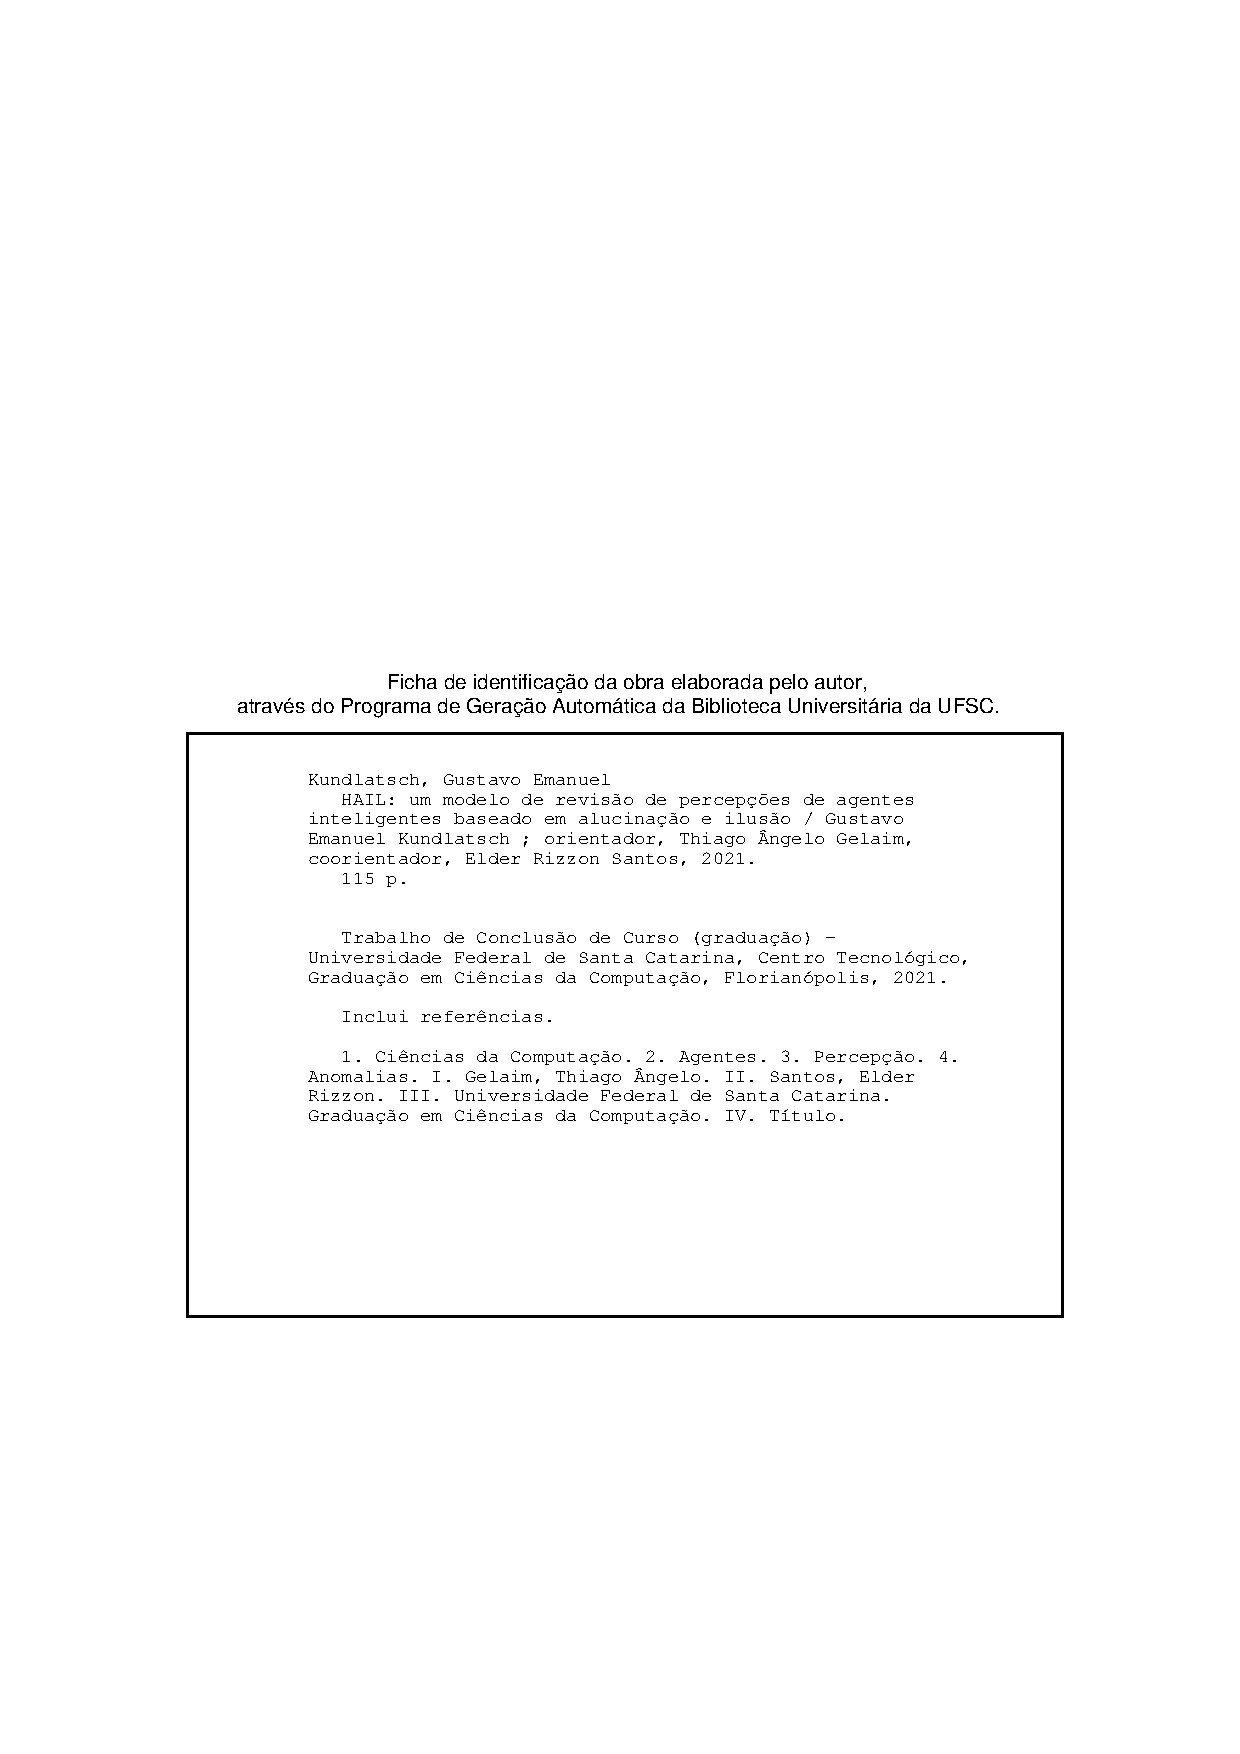
\includepdf{beforetext/Ficha_Catalografica.pdf}
% \end{fichacatalografica}
% ---

% ---
% Inserir folha de aprovação
% ---
% \begin{folhadeaprovacao}
% 	\OnehalfSpacing
% 	\centering
% 	\imprimirautor\\%
% 	\vspace*{10pt}		
% 	\textbf{\imprimirtitulo}%
% 	\ifnotempty{\imprimirsubtitulo}{:~\imprimirsubtitulo}\\%
% 	%		\vspace*{31.5pt}%3\baselineskip
% 	\vspace*{\baselineskip}
% 	%\begin{minipage}{\textwidth}
% 	O presente trabalho em nível de \imprimirnivel~foi avaliado e aprovado por banca examinadora composta pelos seguintes membros:\\
% 	%\end{minipage}%
% 	\vspace*{\baselineskip}
% 	Dr. Thiago Ângelo Gelaim\\
% 	Orientador\\
% 	\vspace*{\baselineskip}
% 	Prof. Dr. Elder Rizzon Santos \\
% 	Coorientador e Responsável\\
% 	\vspace*{\baselineskip}
% 	Prof. Dr. Rafael de Santiago\\
% 	\vspace*{\baselineskip}
% 	Me. Rodrigo Rodrigues Pires de Mello\\
% 	\vspace*{2\baselineskip}
% 	\begin{minipage}{\textwidth}
% 		Certificamos que esta é a \textbf{versão original e final} do trabalho de conclusão que foi julgado adequado para obtenção do título de \imprimirformacao.\\
% 	\end{minipage}
% 	%    \vspace{-0.7cm}
% 	\vspace*{\fill}
% 	\assinatura{\OnehalfSpacing Coordenação do Programa de Graduação}
% 	\vspace*{\fill}
% 	\assinatura{\OnehalfSpacing\imprimirorientador \\ \imprimirorientadorRotulo}
% 	%	\ifnotempty{\imprimircoorientador}{
% 	%	\assinatura{\imprimircoorientador \\ \imprimircoorientadorRotulo \\
% 	%		\imprimirinstituicao~--~\imprimirinstituicaosigla}
% 	%	}
% 	% \newpage
% 	\vspace*{\fill}
% 	\imprimirlocal, \imprimirano.
% \end{folhadeaprovacao}
% ---

% ---
% Dedicatória
% ---
\begin{dedicatoria}
	\vspace*{\fill}
	\noindent
	\begin{adjustwidth*}{}{5.5cm} 
		\raggedleft       
		À Maria, com amor. Minha companheira, amiga e por vezes revisora voluntária. Sua ajuda e motivação fez este trabalho comigo.
	\end{adjustwidth*}
\end{dedicatoria}
% ---

% ---
% Agradecimentos
% ---
\begin{agradecimentos}
    Agradeço a meus orientadores, sem os quais este trabalho não seria possível;
    Aos membros do SpaceLab, em especial a equipe do FloripaSat-2 pela ajuda e suporte;
    À minha família, especialmente minha mãe, que celebrou, reclamou, agradeceu e chorou comigo durante toda a graduação;
    À todos os servidores da UFSC, por manter e prover educação pública, gratuita e de qualidade;
\end{agradecimentos}
% ---

% ---
% Epígrafe
% ---
\begin{epigrafe}
	\vspace*{\fill}
	\begin{flushright}
		\textit{``O êxito precoce é um péssimo professor. Quando isso acontece, somos
                  recompensados por nossa falta de preparação e, quando nos vemos
                  no meio de uma situação para a qual devemos nos preparar, não somos capazes. Não sabemos como fazê-lo.'' \\
			(Chris Hadfield, An Astronaut's Guide to Life on Earth, 2013)}
	\end{flushright}
\end{epigrafe}
% ---

% ---
% RESUMOS
% ---

% resumo em português
\setlength{\absparsep}{18pt} % ajusta o espaçamento dos parágrafos do resumo
\begin{resumo}
	\SingleSpacing
	Satélites artificiais são projetos que demandam níveis elevados de confiabilidade de seus módulos. Apesar de alguns projetos permitirem atualizações posteriores a firmware e programas, são raros os casos onde é possível revisar e corrigir hardware. Por esse motivo a etapa de testes e AIV (\textit{Assembly, Integration, and Verification}) é crucial para a garantia de que o projeto não corra mais riscos do que os que são inerentes à área. Esses fatores são amplificados quando tratamos de \textit{CubeSats}, que possuem escopo e orçamentos menores quando comparados a grandes projetos governamentais e/ou comerciais. Este trabalho propõe a implementação de um sistema de \textit{workflows} hospedados na plataforma de controle de versionamento \textit{GitHub} que, aliados à funcionalidade GitHub Actions, permitirá a execução automatizada de testes no contexto dos planos de \emph{Assembly, Integration, and Verification}(AIV) da missão FloripaSat-2 e, posteriormente, análise e interpretação dos dados coletados de modo a obter resultados qualitativos e quantitativos da execução.
	
	
	\textbf{Palavras-chave}: CubeSat. Nanossatélite. FloripaSat-2. AIV.
\end{resumo}

% resumo em inglês
\begin{resumo}[Abstract]
	\SingleSpacing
	\begin{otherlanguage*}{english}
	    Artificial Satellites are projects that demand highly reliable modules. Despite some missions allowing post-deployment updates to firmware and software, cases where it is possible to perform hardware maintenance are rare. Because of this fact, the \textit{Assembly, Integration and Verification} (AIV) process is crucial to guarantee that the project doesn't face more risks than those which are inerent of a space mission. These factores are intensified when dealing with \textit{CubeSats}, that statistically have lower budgets and scope when compared to large scale governmental and/or commercial space missions. This article proposes the implementation of a test automation workflow system hosted at GitHub that will make use of the GitHub Actions tool to allow automated execution of tests during the AIV step of the FloripaSat-2 mission, and lastly, will allow collection and analysis of data in order to draw relevant conclusions regarding the execution.
	
	
		\textbf{Keywords}: CubeSat. Nanosatellite. FloripaSat-2. AIV.
	\end{otherlanguage*}
\end{resumo}
%% resumo em francês 
%\begin{resumo}[Résumé]
% \begin{otherlanguage*}{french}
%    Il s'agit d'un résumé en français.
% 
%   \textbf{Mots-clés}: latex. abntex. publication de textes.
% \end{otherlanguage*}
%\end{resumo}
%
%% resumo em espanhol
%\begin{resumo}[Resumen]
% \begin{otherlanguage*}{spanish}
%   Este es el resumen en español.
%  
%   \textbf{Palabras clave}: latex. abntex. publicación de textos.
% \end{otherlanguage*}
%\end{resumo}
%% ---

{%hidelinks
	\hypersetup{hidelinks}
	% ---
	% inserir lista de ilustrações
	% ---
	\pdfbookmark[0]{\listfigurename}{lof}
	\listoffigures*
	\cleardoublepage
	% ---
	
	% ---
	% inserir lista de quadros
	% ---
	\pdfbookmark[0]{\listofquadrosname}{loq}
	\listofquadros*
	\cleardoublepage
	% ---
	
	% ---
% 	inserir lista de tabelas
% 	% ---
	\pdfbookmark[0]{\listtablename}{lot}
	\listoftables*
	\cleardoublepage
	% ---
	
	
	% ---
	% inserir lista de abreviaturas e siglas (devem ser declarados no preambulo)
	% ---
	% ---------------------------------------------------
% ------ Lista de abreviaturas e siglas -------------
% ---------------------------------------------------

\begin{siglas}
  \item[ AIV ] \emph{Assembly, Integration, and Verification}
  \item[ CSA ] \textit{Canadian Space Agency}
  \item[ FlatSat ] Plataforma de testes para módulos CubeSat
  \item[ NASA ] \textit{National Aeronautics and Space Administration}
  \item[ SpaceLab ] Laboratório de Pesquisa em Tecnologias Espaciais - UFSC
  \item[ UFSC ] Universidade Federal de Santa Catarina
\end{siglas}
	% ---
	
	% ---
	% inserir lista de símbolos (devem ser declarados no preambulo)
	% ---
% 	% ---------------------------------------------------
% ----------- Lista de símbolos ---------------------
% ---------------------------------------------------

\begin{simbolos}
%   \item[$ \Delta $] Função de transição do modelo de revisão de percepções
%   \item[$ \Gamma $] Função de transição que especifica um sistema de transição de estados $\Sigma$
%   \item[$ \gamma $] Função de percepção do agente
%   \item[$ \theta $] Função de refinamento
%   \item[$ \rho $] Conjunto de percepções refinadas
%   \item[$ \Sigma $] Sistema de transição de estados de um modelo conceitual de planejamento automatizado
%   \item[$ \Psi $] Conjunto união formado pelas pré-condições das ações que compõem um plano
%   \item[$ \psi $] Conjunto de pré-condições de uma ação
%   \item[$ \Omega $] Conjunto união formado pelas pós-condições das ações que compõem um plano
%   \item[$ \omega $] Conjunto de pós-condições de uma ação
%   \item[$ A $] Conjunto finito ou recursivamente enumerável de ações
%   \item[$ Ab $] Conjunto de blocos avaliadores
%   \item[$ Ab_{h} $] Bloco avaliador de alucinações
%   \item[$ Ab_{i1} $] Bloco avaliador de ilusões classe 1
%   \item[$ Ab_{i2} $] Bloco avaliador de ilusões classe 2
%   \item[$ Ag$ ] Agente
%   \item[$ Ap $] Conjunto de blocos de planejamento automatizado
%   \item[$ Ap_{h} $] Bloco de planejamento automatizado de alucinações
%   \item[$ Ap_{i} $] Bloco de planejamento automatizado de ilusões
%   \item[$ c $] Contexto do agente
%   \item[$ Ce $] Função equação de limpeza do bloco avaliador
%   \item[$ Cf $] Função de limpeza do bloco avaliador
%   \item[$ D $] Conjunto de decisores
%   \item[$ d_{a} $] Decisor de anomalias
%   \item[$ d_{h} $] Decisor de alucinações
%   \item[$ d_{i} $] Decisor de ilusões
%   \item[$ E $] Conjunto finito ou recursivamente enumerável de eventos
%   \item[$ K $] Conjunto de conhecimentos do agente
%   \item[$ L $] Lista ordenada
%   \item[$ |L| $] Número de elementos de uma lista ordenada
%   \item[$ L_i $] Elemento $i$ da lista ordenada $L$
%   \item[$ M_{ai} $] Módulo de alucinação e ilusão
%   \item[$ P $] Conjunto de planos do agente
%   \item[$ p $] Conjunto de percepções iniciais
%   \item[$ P(L_i) $] Função peso da lista ponderada
%   \item[$ Pf $] Função de processamento do bloco avaliador
%   \item[$ S $] Conjunto finito ou recursivamente enumerável de estados
%   \item[$ T_{m}(x) $] Função tempo médio de x
%   \item[$ W $] Função peso de uma anomalia
%   \item[$ Z $] Descrição de sistema
\end{simbolos}


	% ---
	
	% ---
	% inserir o sumario
	% ---
	\pdfbookmark[0]{\contentsname}{toc}
	\tableofcontents*
	\cleardoublepage
	
}%hidelinks
% ---
% ---

% ----------------------------------------------------------
% ELEMENTOS TEXTUAIS
% ----------------------------------------------------------
\textual

\chapter{Introdução}
\label{chapter:introducao}
% \section{Introdução}
CubeSats são uma classe de artefatos espaciais elaborada com o intuito de reduzir custos e tempo de desenvolvimento, além de providenciar maior acessibilidade ao espaço \cite{cubesat-spec}. Inicialmente projetados para utilização educacional em universidades \cite{burt2011}, são amplamente usados para exploração espacial em órbita terrestre baixa, com altitudes entre 160km e 2000km \cite{alanazi2019}.

CubeSats possuem uma unidade básica (U) de dimensão 10cm x 10cm x 10cm e de até 1kg de massa, mas podem ser configurados em até 24 Unidades (ou 24U) \cite{cubesat}. O FloripaSat-2 \cite{floripasat2}, projeto do Laboratório de Pesquisa em Tecnologias Espaciais da UFSC no qual este trabalho se baseia, é um CubeSat 2U que se encontra no presente momento, em estágio de desenvolvimento ativo. A figura \ref{fig:floripasat2-diagram} apresenta uma renderização da configuração do FloripaSat-2.

\begin{figure}[H]
\caption{\label{fig:floripasat2-diagram}Renderização do FloripaSat-2.}
\begin{center}
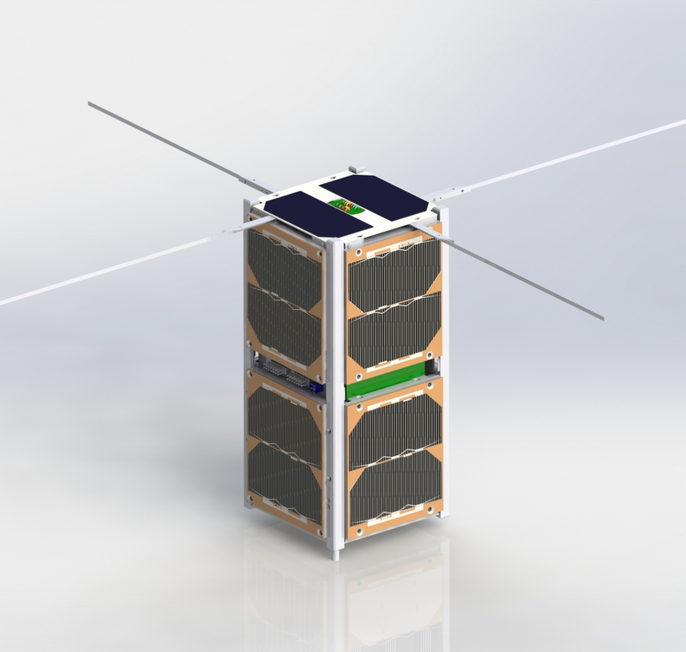
\includegraphics[scale=0.5]{images/floripasat-2-diagram.jpg}
\end{center}
\legend{Fonte: \cite{floripasat2}}
\end{figure}
\newpage

O processo de verificação de design é uma etapa crucial em projetos de engenharia.
Em tradução livre dos autores, Monteiro et al, dizem que:

\begin{citacao}
\hspace{1,2cm}Em projetos espaciais, a amplitude e cuidado minucioso dos processos de teste são ainda mais importantes, em vista do nível de confiabilidade  a ser imposto no produto final, que é comumente um artefato espacial que precisa resistir à uma gama de ameaças e funcionar em um ambientes inóspitos. \cite{aiv-cubesat}
\end{citacao}

Ainda segundo os autores, o processo de \emph{AIV} (sigla em inglês para Montagem, Integração, e Verificação) tende a ser mais leve em CubeSats, devido à menor escala dos projetos.

No entanto, o risco de um projeto de nanossatélite não é desprezível. Em um estudo realizado sobre os lançamentos de CubeSats entre 2003 e 2015, os autores \cite{panga2016} constataram que cerca de 15\% das missões CubeSat nesse período não conseguiram manter comunicações com as estações de controle, resultando em falha da missão após o lançamento.

Por esses motivos, percebe-se então a relevância de um plano de testes bem estruturado para o ciclo de desenvolvimento do FloripaSat-2. Através da elaboração e execução de testes, pretende-se elevar a confiabilidade\cite{chen-2001} do sistema, a fim de diminuir a probabilidade de que problemas no satélite resultem em falha da missão


O trabalho propõe, então, dois pontos principais:

\begin{itemize}
    \item A implementação de um sistema de workflows hospedados na plataforma GitHub Actions \cite {gh-actions} nos repositórios oficiais do projeto, que possibilite a execução automática de testes unitários nos sistemas do FloripaSat-2;
    \item A análise desritiva dos testes unitários implementados durante o desenvolvimento dos subsistemas do satélite.
\end{itemize}

Os resultados esperados deste trabalho são a criação de um modelo para automação a ser usado em futuros projetos de desenvolvimento de sistemas embarcados para CubeSats, e um relatório com as conclusões e análises obtidas por meio do estudo dos dados coletados.

\section{Objetivos}

\subsection{Objetivo Geral}

O objetivo principal do trabalho é implementar um sistema de automação dos testes unitários do firmware do FloripaSat-2 hospedado nos repositórios oficiais no \textit{GitHub}. Esses \textit{workflows} serão empregados durante o ciclo de desenvolvimento da missão, executando os testes de forma automática seguindo os critérios de execução estabelecidos pelo projeto.

\subsection{Objetivos Específicos}

\begin{enumerate}
    \item Apresentar uma introdução ao estado da arte referente a testes de software, desenvolvimento de CubeSats e relacionar os dois temas no contexto do FloripaSat-2;
    \item Implementar \textit{workflows} capazes de automatizar a execução de testes unitários;
    \item Apresentar um estudo sobre os testes dos sistemas do FloripaSat-2 que foram implementados durante o andamento do projeto;
    \item Disponibilizar códigos-fonte, dados de registro e resultados obtidos.
\end{enumerate}
\section{Organização do trabalho}

Este trabalho está organizado do seguinte modo:

\begin{itemize}
    \item O capítulo \ref{chapter:fundamentacao} apresenta a definição da metodologia utilizada e a formalização da fundamentação teórica utilizada na elaboração do trabalho;
    \item O capítulo \ref{chapter:relacionados} apresenta uma breve revisão de alguns trabalhos relacionados que abordam o desenvolvimento e testes de CubeSats;
    \item O capítulo \ref{chapter:proposta} apresenta e descreve o sistema proposto;
    \item O capítulo \ref{chapter:projeto} apresenta a descrição formal da implementação do sistema
    \item O capítulo \ref{chapter:resultados} apresenta uma análise dos resultados observados
    \item O capítulo \ref{chapter:conclusao} traz as conclusões e considerações sobre o trabalho, e explora possíveis trabalhos futuros
\end{itemize}

\chapter{Fundamentação teórica}

\label{conceitos-fundamentais}
Este capítulo apresenta a fundamentação teórica utilizada na elaboração do trabalho, trazendo conceitos básicos de nanossatélites
e automação de testes, além de um aprofundamento sobre como os temas foram empregados durante o desenvolvimento e implementação do trabalho.

\section{CubeSat}
\label{section:cubesat}
CubeSats são uma categoria de satélites miniaturizados cuja principal característica é possuir dimensões e massa reduzidos.
De acordo com o documento oficial de padrões de design\cite{cubesat-spec}, CubeSats devem ter estrutura em formato de cubo de
lado 100mm e não podem exceder 1kg de massa.

Essas características correspondem a uma unidade, ou um CubeSat 1U. Cubesats podem ser empilhados em múltiplas unidades, em
configurações como 2U, 3U, 6U ou 12U.

O padrão CubeSat foi desenvolvido pela \textit{California Polytechnic State University}, e é uma especificação de projeto de
colaboração internacional entre governos, universidades, escolas e o setor privado, com o principal objetivo de conceder acesso
ao espaço para cargas pequenas, e possibilitar missões com objetivos diversos, como demonstrações de tecnologia, como foi o caso
da missão Mars Cube One, desenvolvida pelo Jet Propulsion Laboratory e enviada à Marte \cite{mars-cubesat}, ou com objetivos
educacionais, como os CubeSats desenvolvidos pelo SpaceLab da UFSC.

Os CubeSats tradicionalmente possuem custo e risco baixos. Por serem fabricados em sua maioria com peças e materiais provienientes
de indústriais comvencionais, o orçamento de uma missão não se compara aos orçamentos bilionários de missões convencionais.
E do mesmo modo, o risco de se perder um CubeSat em uma missão que resulte em falha não é tão impactante em termos orçamentários e
de trabalho perdido. Esse fato faz com que esse tipo de missão seja ideal para ser utilizado com propósitos educativos por instituições
de ensino. A missão FloripaSat-1 da UFSC, por exemplo, teve como um dos objetivos treinar e capacitar estudantes de engenharia no processo
de desenvolvimento e operação de uma missão espacial \cite{marcelino2020-1}.

\section{Teste de Software}
Segundo Raul Wazlawick, quando se trata de teste é importante definir termos que, apesar de parecerem sinônimos, tem significados distintos
na área de testes de software:

\begin{itemize}
    \item error (error)
    \item defeito (fault)
    \item falha (failure)
    \item engano (mistake)
\end{itemize}

\section{CMocka}
CMocka is an elegant unit testing framework for C with support for mock objects. It only requires the standard C library,
works on a range of computing platforms (including embedded) and with different compilers.

\section{Mockups}
Mockups

\section{Automação de Testes}
\label{section:test-automation}

Durante o tempo de vida de um projeto de um software ou um sistema de softwares, como é o caso de um projeto de satélites artificiais,
os componentes envolvidos invariavelmente passarão por algumas mudanças. Mudanças essas que podem introduzir novos \textit{bugs} em
componentes que anteriormente funcionavam. A automação de testes, como definido pelos autores do livro
\textit{Software Test Automation - Effective use of test execution tools}, se dá pelo emprego de tecnologias que permitam que um caso
de teste seja executado de maneira autônoma, sem intervenção ou monitoramento, de maneira muito mais eficiente\cite{software-automation}
do que se executado via interação humana.

A etapa de testes é essencial em qualquer projeto de engenharia, e pode-se dizer que é ainda mais importante em projetos espaciais, já
que erros de projeto, sejam eles de hardware ou firmware, podem resultar em falha da missão.

Este trabalho propõe adotar a ferramenta de automação de testes em uma missão CubeSat, mais específicamente a FloripaSat-2, desenvolvida
pelo laboratório SpaceLab da Universidade Federal de Santa Catarina.

A FloripaSat-2 utilizará para testar e validar os seus subsistemas uma \textit{FlatSat}, descrita com mais detalhes na seção
\ref{section:flatsat}. O uso de \textit{FlatSats} tem um bom histórico de auxiliar na detecção e correção de erros e \textit{bugs},
como descrito por \cite{aiv-cubesat} e \cite{marcelino2020-2}. Por isso, julga-se que os bons resultados podem ser potencializados
por uma ferramenta de automação de testes, que permitirá a adoção de uma estratégia iterativa de desenvolvimento e correção de erros.

% \chapter{Trabalhos Relacionados}
\chapter{Trabalhos relacionados}

\label{chapter:relacionados}

No motor de pesquisa acadêmica Google Scholar foram feitas pesquisas associando as áreas de conhecimento de desenvolvimento de nanossatélites, testes de software e automação de testes. As pesquisas foram realizadas ao longo da elaboração do trabalho e diferentes \textit{strings} de busca foram utilizadas. Como critério para escolha das publicações à serem estudadas, foram analisados os resultados apresentados na primeira página do motor de busca. Para determinar a relevância de uma publicação para o trabalho, foi analisado o \textit{abstract} e a introdução dos mesmos.

% A popularidade dos CubeSats cresce anualmente, com cada vez mais lançamentos realizados. Por esse motivo, existem inúmeros artigos, com mais sendo publicados constantemente.

\begin{quadro}[]
\caption{Pesquisas realizadas}
\begin{tabular}{|l|l|}
\hline
\textit{String}          & Resultados \\ \hline
nanosattelite + design   & 15,200     \\
software + test          & 4,300,000  \\
software+test+automation & 1,970,000  \\
flatsat + cubesat        & 359        \\
cubesat                  & 29,200     \\
flatsat + nanosatellite  & 273        \\
cubesat + testbed        & 3,510      \\ \hline
\end{tabular}
 \label{tab:pesquisas}
 \legend{Fonte: Autor.}
\end{quadro}

% Existem diversas abordagens para otimizar as percepções recebidas por um agente, isto é, garantir que todas as informações coletadas pelos sensores sejam utilizadas da melhor maneira possível. Diversos artigos sobre o assunto, com diferentes abordagens, são publicados todos os anos. Para definir os trabalhos relacionados apresentados nessa seção, foram utilizados diversos termos de busca, uma vez que os termos ilusão e alucinação podem não necessariamente se aplicarem às percepções da mesma maneira definida neste trabalho.

% Nos mecanismos de busca Google Scholar e Scopus foram realizadas pesquisas que associam agentes inteligentes a percepções inválidas, anomalias ou ilusões e alucinações, além de termos auxiliares como aprendizado e otimização. As buscas aconteceram ao longo do desenvolvimento do trabalho, e diversas \textit{strings} de busca foram utilizadas e combinadas. Conforme encontraram-se os artigos, suas introduções foram verificadas para averiguar se o conteúdo realmente estava relacionado ao processo de revisão de percepções. Depois disso foi realizada uma leitura inicial dos trabalhos selecionados, e os quatro mais adequados foram escolhidos para um estudo mais profundo.

% Os artigos apresentados nas Seções \ref{van2011} e \ref{diab2019} implementam modelos para tratar de percepções em ambientes onde é possível receber percepções que não são totalmente confiáveis, semelhante ao conceito de anomalia definido no Capítulo \ref{conceitos-fundamentais}. Os artigos das Seções \ref{pangercic2010} e \ref{kim2017} são trabalhos relacionados a outros campos de estudo de percepção, mas que precisam resolver problemas relacionados a percepções imperfeitas. A maneira como esses artigos se conectam ao modelo proposto no trabalho atual está descrita em mais detalhes nas seções seguintes.


\section{Integration and Verification Approach of ISTSat-1 CubeSat \\ \cite{aiv-cubesat}}
\label{aiv-cubesat}
Satélites artificiais precisam resistir a uma grande quantidade de adversidades enquanto operam em um ambiente hostil e inóspito. Por isso é essencial que sejam feitos testes extensivos para garantir o nível de confiança necessário para que o objetivos da missão sejam atingidos. Porém, missões de CubeSat tendem a não ser tão rigorosas em suas etapas de montagem, integração e verificação (AIV), fato que é refletido na taxa de missões que acabam em falhas.

Esse paradigma, no entanto, está mudando a medida que a importância do CubeSats aumenta. Ela vai de simplesmente projetos educacionais, para missões de custos e importância elevados. Um exemplo desse salto é a missão Mars Cube One, ou MarCO \cite{mars-cubesat}, desenvolvida pelo \textit{Jet Propulsion Laboratory} da Nasa, que enviou dois CubeSats a Marte, para servirem como satélites de comunicação. Assim, os autores desse artigo apresentam a ideia de que integração e verificação em missões CUbeSats passam a ser encaradas com mais seriedade, como demonstrado na figura \ref{fig:nanosats_years_forecast}, onde é possível observar o aumento de lançamento de nanossatélites e, paralelamente, a diminuição da taxa de falhas.

Como estudo de caso, o artigo apresenta o processo de AIV empregado no desenvolvimento do ISTSat-1 \cite{istsat-1}, o primeiro nanossatélite português, lançado em 2021 e que utilizou a estratégia de teste através de uma \textit{FlatSat}, que se trata de uma plataforma de testes de \textit{Hardware In the Loop} (HIL).

A equipe do ISTSat-1, segundo os autores, optou por desenvolver a maioria dos subsistemas do satélite e adotou métodos ágeis para as atividades de AIV de forma a diminuir os riscos relacionados a falta de experiência da equipe. Dessa forma foi possível desenvolver e testar os módulos de forma contínua e iterativa, o que possibilitou a descoberta rápida de diversos erros e problemas que necessitavam de ajustes de design. Foi concluído nesse estudo que, caso a equipe tivesse optado por um processo de desenvolvimento em cascata, como tradicionalmente empregado em missões CubeSat, seria mais difícil, senão impossível, ter descoberto os mesmos problemas no design e funcionamento. Concluem então, que a adoção de processos iterativos é útil para projetos educacionais que contam com equipes sem muita experiência, ou sem muitos recursos financeiros.

\begin{figure}[h!]
    \centering
    \caption{Lançamentos anuais de Nanossatélites (previsão)}
    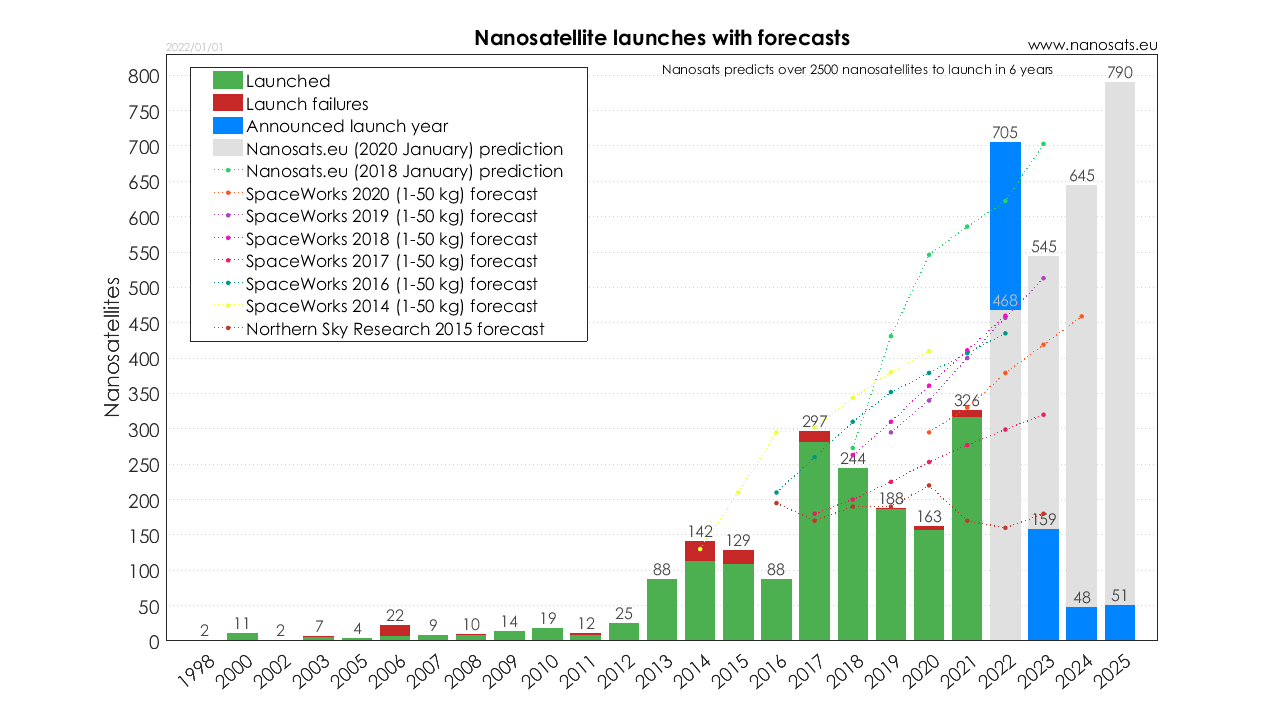
\includegraphics[width=\textwidth]{images/nanosat_years_forecast.png}
    \legend{Fonte: Nanosats Database \cite{nanosats-database}}
    \label{fig:nanosats_years_forecast}
\end{figure}


\section{Qualification and validation test methodology of the
open-source CubeSat FloripaSat-I \cite{marcelino2020-2}}

Esta seção e a próxima apresentam dois trabalhos produzidos como resultado da missão FloripaSat-1, uma missão de demonstração desenvolvida inteiramente por estudantes da Universidade Federal de Santa Catarina (UFSC), cujo CubeSat foi lançado em 2019.

O FloripaSat-1 é composto de três módulos distintos, o sistema elétrico - EPS (\textit{Electric Power System}), o módulo de gerência de dados - OBDH (\textit{Onboard Data Handling}) e o módulo de telemetria e telecomandos - TT\&C (\textit{Telemetry, Tracking and Command}).

O artigo informa que a missão tinha como objetivo testar tecnologias que possibilitem o desenvolvimento rápido e de baixo custo de satélites espaciais, além de treinar estudantes nas áreas de concepção, implementação e operação de uma missão espacial completa. Além disso, o FloripaSat-1 é um projeto \textit{open source} e as informações de software e hardware dos módulos desenvolvidos estão disponíveis em repositórios públicos, para uso em futuras missões.

Os autores descrevem que o FloripaSat-1 foi desenvolvido com base em projetos de engenharia de sistemas, dividido em Modelos de protótipo (PM), engenharia (EM-I e EM-II) e finalmente o Modelo de Vôo (FM). Foram realizados testes em cada uma dessas etapas para validar os sistemas e os resultados, segundo o artigo, foram decisivos na detecção e correção de erros.

Apesar do artigo focar em integração e validação dos módulos a nível de hardware, julga-se relevante para a elaboração deste trabalho, que foca principalmente em software, por descrever as diferentes condições que uma missão espacial é submetida, além da metodologia de desenvolvimento adotada pela equipe do FloripaSat-1, em que a grande maioria dos membros seguiu para a missão FloripaSat-2, a qual este trabalho se baseia.

\section{A Critical Embedded System Challenge: The
FloripaSat-1 Mission \cite{marcelino2020-1}}

Este artigo, elaborado também a partir da missão FloripaSat-1 do SpaceLab, apresenta definições e descrições dos subsistemas do satélite, além de algumas informações e resultados de testes e simulações realizadas nos mesmos.

Como descrito anteriormente, o FloripaSat-1 possui três sub sistemas principais:

\begin{itemize}
    \item \textit{Electric Power System} (EPS)
    \item \textit{On-Board Data Handling} (OBDH)
    \item \textit{Tracking, Telemetry and Command} (TT\&C)
\end{itemize}

O EPS é o módulo responsável por distribuir, coletar e armazenar a energia utilizada pelo satélite. A energia é coletada através de painéis solares e armazenada em uma bateria de íon de lítio. A distribuição da energia é definida a partir de um microcontrolador que analisa os estados de carga e de energia e decide quais módulos permanecerão em operação.

O OBDH é o módulo responsável pela gerência de atividades do satélite. Ele realiza a interface entre todos os subsistemas do satélite. Os dados gerados são empacotados e transmitidos através do TT\&C, e dados recebidos são enviados ao OBDH para que ele execute a tarefa requisitada, ou então envie o comando ao módulo requisitado. Este módulo também possui uma memória, para que possam ser futuramente recuperados.

Finalmente, o TT\&C é o módulo responsável pela comunicação entre o satélite e as estações de controle na Terra. Ele opera através de dois módulos de rádio, um para a banda VHF e um para UHF. Os comandos a serem enviados e recebidos pelo satélite (\textit{downlink}/ \textit{uplink}) são transmitidos através do módulo UHF e a banda VHF é reservada para transmissões do tipo \textit{beacon}.

Os autores discorrem ainda sobre os demais módulos e subsistemas do satélite, como outros \textit{payloads} que não foram desenvolvidos ou projetados pela equipe da UFSC e portanto, ficam de fora desse breve resumo.

A relevância deste artigo se dá pelo fato de que o FloripaSat-2 utiliza a mesma estrutura de subsistemas, com os seus módulos sendo sucessores diretos do software e hardware utilizados na missão anterior, operando de forma idêntica ou muito similar.


%

\section{Considerações}

Os trabalhos relacionados escolhidos têm como principal função estabeler a importância de uma estrutura de testes bem fundamentada. Todos os trabalhos mencionam que a etapa de testes foi importante pra a descoberta e solução de erros que não foram descobertos ou detectados durante os ciclos de desenvolvimento normais.

Além disso, os dois trabalhos produzidos por estudantes do SpaceLab como resultado da missão FloripaSat-1 mostram a importância de CubeSats como ferramenta educacional, servindo para treinar e capacitar estudantes no projeto, desenvolvimento e operação de uma missão espacial completa.

O modelo proposto por este trabalho é uma continuidade desse pensamento: possibilitar mais uma ferramenta de testes que possa resultar em maior confiabilidade dos sistemas embarcados desenvolvidos para o FloripaSat-2, fazendo uso do ambiente de aprendizado e da experiência adquirida durante o desenvolvimento da missão.

\iffalse

\fi
\chapter{Proposta}
\label{chapter:proposta}

Este capítulo descreve e formaliza o sistema proposto por este trabalho. A motivação para este trabalho surgiu a partir de conversas e reuniões com as equipes de desenvolvimento do FloripaSat-2, e tem como inspiração projetos que utilizam conceitos de integração contínua para automatizar o processo de testes e \textit{deploy} de sistemas.

Inicialmente, como teste de conceito, foi criado um \textit{workflow} para automatizar a execução dos testes dos programas de alguns dos subsistemas do satélite, porém, foi feito de um modo genérico o suficiente para que pudesse ser implementado em todos os outro módulos do FloripaSat-2.

Após verificar o funcionamento e a utilidade destes \textit{workflows}, surgiu a possibilidade de aplicar os mesmos conceitos à FlatSat da missão, de modo a automatizar os testes de software e assim, esta se tornou oficialmente a proposta do trabalho.

Os workflows propostos por este trabalho seguirão a mesma linha de raciocínio e apresentarão funcionalidades semelhantes aos já implementados. As próximas seções apresentam uma descrição do modelo proposto, fazendo comparações, quando possível, com o que já foi implementado.


\section{visão geral}
A \textit{FlatSat}, como descrita na seção \ref{section:flatsat}, é uma maneira de testar de maneira rápida e simultânea os subsistemas do satélite. Esta proposta foca em testes de software, utilizando a flatsat como ferramenta de acesso aos sistemas embarcados. Através dela, será possível testar os programas embarcados do FloripaSat-2 de maneira simultânea e em conjunto, analisando a interação entre os diferentes substistemas, além dos funcionamentos isolados.

Estes \textit{workflows} ainda estão em fase de concepção durante a elaboração deste TCC. Por isso, as próximas seções se baseiam nos fluxos de execução já implementados, que possuem muitos dos mesmos objetivos e características de funcionamento.

\section{Workflows}
Esta seção e a próxima tomam como exemplo os workflows de automação empregados no módulo OBDH 2.0, já que os fluxos de automação específicos para a FlatSat serão estruturados de maneira similar e seguindo os mesmos principios. Esta seção apresenta algumas seções de código extraídas para ilustrar e demonstrar o funcionamento do sistema, mas os códigos estão disponíveis de forma pública nos repositórios dos subsistemas, como \cite{eps2-github} e \cite{obdh2-github}. Eles também são apresentados integralmente ao final deste documento, no Apdêndice \ref{cod:obdh_devices}.

    \subsection{Identificação dos Arquivos}
    Os \textit{workflows} são responsáveis por executar uma bateria de testes de unidade, que estão separados em arquivos únicos. Inicialmente, o sistema precisa identificar e compilar cada um desses arquivos de teste. Para isso é empregado um script \textit{Python} que procura nas localizações relevantes arquivos que possuam a nomenclatura apropriada. Neste caso, arquivos cujos nomes terminam como \textit{\_test.c}. O trecho de código abaixo, extraído do arquivo \textit{deployJSON.py} e disponível em \ref{deployJSON.py}, demonstra essa busca pelos arquivos relevantes.

    Os nomes e localização dos testes encontrados são salvos em um arquivo \textit{.json}, utilizado posteriormente para compilação.
    \begin{minted}
        [
        frame=lines,
        framesep=2mm,
        baselinestretch=1.2,
        breaklines=True,
        fontsize=\footnotesize,
        linenos
        ]
        {python}
        for file in file_dir:
        if file.endswith('_test.c'):
            file_name = file.replace('.c', '')
            test_file = file_name.replace('_test', '_unit_test')
            file_path = path + test_file

            file_info = {
                "name": file_name,
                "test_name": test_file,
                "path": file_path
            }

            files['include'].append(file_info)
    \end{minted}

    \subsection{\textit{Job Matrix}}
    Para garantir que os testes sejam executados com relativa rapidez, o \textit{workflow} foi estruturado para executar cada teste simultaneamente de forma isolada. Para isso, foi utilizada uma \textit{Job Matrix}, que se trata de uma maneira de dividir um \textit{workflow} em subtarefas que se excutam paralelamente. Uma explicação detalhada do funcionamento e configuração de uma \textit{Job Matrix} pode ser encontrada na documentação oficial da ferramenta \textit{GitHub Actions} \cite{gh-actions}.

    Neste caso, o número de subtarefas, ou \textit{jobs}, é definido pela quantidade de testes que foram encontrados pelo passo anterior, para que assim o \textit{workflow} gere a matriz através do resultado da execução do script apresentado anteriormente. O Trecho de código a seguir apresenta essa funcionalidade.

    \begin{minted}
        [
        frame=lines,
        framesep=2mm,
        baselinestretch=1.2,
        breaklines=True,
        fontsize=\footnotesize,
        linenos
        ]
        {yaml}

    generate-matrix:
        name:

        runs-on: ubuntu-latest

        outputs:
          matrix: ${{ steps.set-matrix.outputs.matrix }}

        steps:
          # Checks-out the repository under $GITHUB_WORKSPACE, so the job can navigate it
          - uses: actions/checkout@v2

          - name: Create JSON file
            run: python3 .github/workflows/deployJSON.py --source firmware/tests/devices/

          - name: Resulting JSON file for matrix generation
            run: echo "$(cat .github/workflows/test-list.json)"

          # Set the matrix output from the JSON (manipulated to remove spaces and replace \n -> %0A, " -> \")
          - id: set-matrix
            name: Set matrix output from the JSON file
            run: echo "::set-output name=matrix::$( echo "$(cat .github/workflows/test-list.json)" | sed ':a;N;$!ba;s/\n/%0A/g' )"

    \end{minted}


    \subsection{Compilação e execução}
    A compilação é feita através de um comando \textit{make}, recebendo como entrada cada um dos arquivos encontrados pelo script identificador. A Matriz de subtarefas é organizada de modo que os arquivos sejam divididos de maneira única, ou seja, cada subdivisão do \textit{workflow} é responsável por compilar e executar um único teste.
    A figura \ref{fig:workflow_execution_diagram} apresenta um diagrama exemplificando o fluxo de execução do processo descrito. O diagrama não representa a identificação dos arquivos de teste.

    \begin{figure}[!ht]
        \centering
        \caption{Diagrama de execução de um workflow de testes automatizados}
        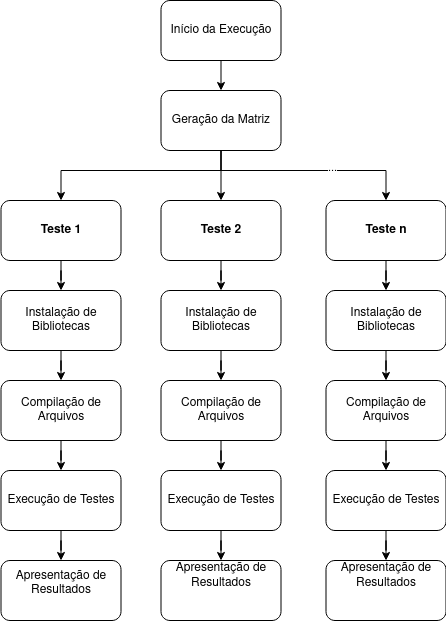
\includegraphics[width=0.8\textwidth]{images/Workflow Execution.drawio.png}
        \legend{Fonte: Autor}
        \label{fig:workflow_execution_diagram}
    \end{figure}

    % \begin{minted}
    % [
    % frame=lines,
    % framesep=2mm,
    % baselinestretch=1.2,
    % breaklines=True,
    % fontsize=\footnotesize,
    % linenos
    % ]
    % {yaml}
    % \end{minted}

\section{\textit{GitHub Actions}}
Esta seção apresenta uma breve descrição da ferramenta \textit{GitHub Actions}, cuja documentação oficial e completa está disponível em \cite{gh-actions}. Ela se uma plataforma de CI/CD (\textit{Continuous Integration/Continuous Delivery}) que permite automatizar testes, builds e deploys através da execução de \textit{workflows} que realizam essas tarefas após alterações no repositório como \textit{commits}, ou \textit{pull requests}.

    \subsection{Hospedagem}
    Os servidores responsáveis pela execução dos \textit{workflows} são chamados de \textit{runners}. O \textit{GitHub} fornece servidores Windows, Ubuntu e macOS, e cada execução de um workflow ocorre em uma máquina virtual nova. Também é possível usar um servidor próprio, chamados de servidores \textit{self-hosted}. Os \textit{workflows} implementados até o momento são executados em servidores Ubuntu do \textit{GitHub}. Os implementados para a FlatSat, no entanto, serão executados em servidores \textit{self-hosted}, já que será necessário manter conexão com os módulos do FloripaSat-2 de modo a testar e executar os programas embarcados.

    \subsection{Execução}
    É possível planejar a execução dos \textit{workflows} e sincronizá-las com ações dentro dos repositórios. Nos casos do OBDH 2.0 e do EPS 2.0, os testes são executados após \textit{commits} em \textit{branches} específicas do repositório como a \textit{master} ou \textit{dev-firmware}, ou após \textit{pull requests}. Também é possível configurar a execução manual, para executar os testes sem realizar nenhuma alteração prévia no repositório.

    \subsection{Resultados}
    Ao fim da execução dos \textit{workflows}, a ferramenta apresenta um \textit{log} com todos os eventos e mensagens retultantes da execução. Aqui é possível, por exemplo, verificar se houve alguma falha na execução dos testes. Esses registros ficam disponíveis no repositório, e sua utilidade vem do nível de detalhamento que forem configurados. Para o sistema proposto por este trabalho, espera-se um elevado nível de detalhamento dos registros, de modo que os resultados possam ser analisados e seja possível extrair dados conclusivos sobre dados de execução e estatística de falhas e sucessos nos testes. A figura \ref{fig:workflow_log} apresenta uma captura de tela de uma execução dos testes durante um \textit{commit} no repositório do OBDH 2.0.

    \begin{figure}[h!]
        \centering
        \caption{Captura de tela do resultado de uma execução de testes automáticos}
        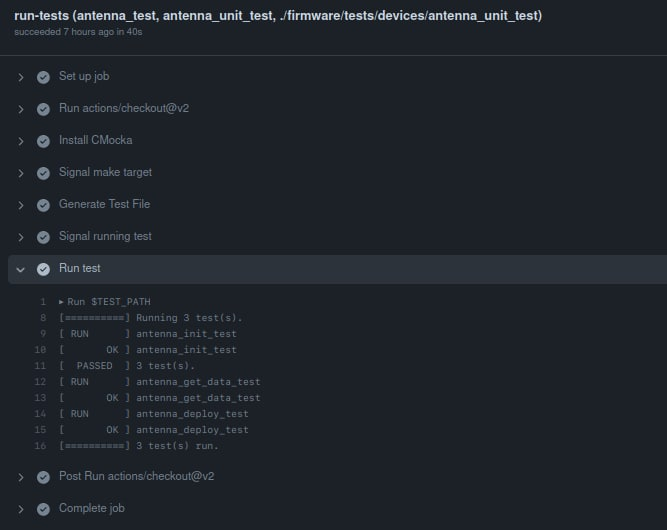
\includegraphics[width=0.9\textwidth]{images/workflow_log.jpg}
        \legend{Fonte: OBDH 2.0 \cite{obdh2-github}}
        \label{fig:workflow_log}
    \end{figure}

\section{Resultados esperados}
Os \textit{workflows} de automação descritos anteriormente se provaram benéficos para o ciclo de desenvolvimento dos sistemas do FloripaSat-2. Através deles, é possível testar cada alteração proposta de maneira eficiente e a automação fornece um registro de execuções passadas, onde é possível comparar alterações no código e os resultados que elas provocaram na execução dos testes. Em termos de controle de versão, os testes foram centralizados e disponibilizados para visualização e estudos.

Espera-se que os programas sob teste na FlatSat possam receber os mesmos benefícios e que isso seja potencializado, visto que o escopo da FlatSat é maior, sendo possível testar não somente a execução individual dos sitemas embarcados, mas também todas as funcionalidades que dependem da integração entre os módulos. Dessa forma, será possível, a princípio, testar o software do FloripaSat-2 como um todo, assumindo que todos os seus substistemas estejam conectados à FlatSat.

Os \textit{workflows} projetados seguirão os mesmos princípios dos que foram descritos anteriormente, de forma a padronizar o uso o dentro da missão e para que seja possível aplicar os mesmos princípios de agilidade e eficiência.

Uma vez que o sistema esteja implementado, espera-se que seu uso contínuo gere uma quantidade considerável de registros e históricos de execução, que serão estudados para produzir a seção de análise deste projeto que trará então um levantamento sobre a utilidade e o impacto do uso desse sistema para o desenvolvimento da missão.

% \input{chapters/5-formalizacao}
% \input{chapters/6-experimentos}
\chapter{Conclusões}

Os trabalhos relacionados escolhidos apresentam um panorama inicial bastante informativo, quando analizados em conjunto:
\begin{itemize}
    \item A relevância de missões CubeSat cresce a cada ano, observada pelo crescente volume de lançamentos;
    \item São projetos com potencial educacional elevado, sendo usados por insituições de ensino para capacitar e treinar estudantes e também desenvolver, testar novas tecnologias e processos de desenvolvimento.
\end{itemize}
 
 Os dois artigos elaborados pela equipe do FloripaSat-1 demonstram a enorme quantidade de conhecimento gerada, bem como a experiência adquirida em projeto e desenvolvimento de tecnologias espaciais.

Percebeu-se também que, embora exista uma biblioteca ampla sobre testes de hardware de \textit{CubeSats}, a quantidade de material distinto que foque apenas (ou principalmente) em teste de software espacial é comparativamente menor. Espera-se que esse trabalho seja, então, uma boa fonte de informação sobre o potencial que esta área pode apresentar para estudos e inovação.

O estudo destes trabalhos relacionados evidência também a importância de um projeto de testes estruturado. Mais de uma vez, nos artigos selecionados anteriormente foi descrito que a etapa de testes foi importante para a descoberta e correção de erros de design, sejam eles de harware ou software. É nessa vertente que este trabalho propõe uma nova aproximação para os testes de software, por meio de um sistema de workflows que permita a execução de testes de maneira automática, fazendo uso da \textit{FlatSat} da missão FloripaSat-2 para testar de maneira simultânea, os sistemas embarcados de todos os módulos do satélite, bem como as interações e comunicações entre eles.

Se bem sucedido, esse modelo potencializará a descoberta e correção de erros e possibiliatará o desenvolvimento de programas mais confiáveis e de forma mais rápida.


\section{Trabalhos Futuros}
Como sugestão e planejamento de trabalhos futuros, sobretudo dando continuidade à este relatório durante a disciplina de Trabalho de Conclusão de Curso II, sugere-se alguns pontos de aprofundamento:
\begin{itemize}
    \item Aprofundar a pesquisa sobre testes de software, trazendo uma breve análise do estado da arte;
    \item Trazer mais trabalhos relacionados sobre testes de software embarcado, e software para aplicações espaciais;
    \item Implementar e apresentar o sistema de \textit{workflows} à ser utilizado em conjunto com a FlatSat do FLoripaSat-2;
    \item Armazenar, preservar, e analisar os registros e histórico de execuções dos fluxos de testes automatizados;
    \item Redigir um estudo de caso trazendo as principais informações e conclusões, tendo como base os dados coletados.
\end{itemize}

% ----------------------------------------------------------
% ELEMENTOS PÓS-TEXTUAIS
% ----------------------------------------------------------
\postextual
% ----------------------------------------------------------

% ----------------------------------------------------------
% Referências bibliográficas
% ----------------------------------------------------------
\begingroup
\printbibliography[title=REFERÊNCIAS]
\endgroup

% ----------------------------------------------------------
% Glossário
% ----------------------------------------------------------
%
% Consulte o manual da classe abntex2 para orientações sobre o glossário.
%
%\glossary

% ----------------------------------------------------------
% Apêndices
% ----------------------------------------------------------

% ---
% Inicia os apêndices
% ---
\begin{apendicesenv}
%	\partapendices*
	% ----------------------------------------------------------
\chapter{\textit{Workflow} de testes de unidade para o módulo OBDH 2.0}
% ----------------------------------------------------------
\label{cod:obdh_devices}
Este capítulo apresenta os códigos necessários para a execução do \textit{workflow} de automação de testes de unidade do módulo OBDH 2.0 \cite{obdh2-github} do FloripSat-2

\begin{section}{unit-tests-devices.yml}
\label{unit-tests-devices.yml}
    \begin{minted}
    [
    frame=lines,
    framesep=2mm,
    baselinestretch=1.2,
    breaklines=True,
    fontsize=\footnotesize,
    linenos
    ]
    {yaml}

#
# unit-tests-devices.yml
#
# Copyright (C) 2021, SpaceLab.
#
# This file is part of OBDH 2.0.
#
# OBDH 2.0 is free software: you can redistribute it and/or modify
# it under the terms of the GNU General Public License as published by
# the Free Software Foundation, either version 3 of the License, or
# (at your option) any later version.
#
# OBDH 2.0 is distributed in the hope that it will be useful,
# but WITHOUT ANY WARRANTY; without even the implied warranty of
# MERCHANTABILITY or FITNESS FOR A PARTICULAR PURPOSE. See the
# GNU General Public License for more details.
#
# You should have received a copy of the GNU General Public License
# along with OBDH 2.0. If not, see <http://www.gnu.org/licenses/>.
#
#


name: Devices Unit Tests

on:
  push:
    branches: [ dev_firmware ]
  pull_request:
    branches: [ master, dev, dev_firmware]

  # 'workflow_dispatch' allows manual execution
  # of this workflow under the repository's 'Actions' tab
  workflow_dispatch:

jobs:

  # Generates Matrix
  # This job executes the 'deployJSON.py' script
  # which compiles a list of all files ending in '_test.c'
  # in a given directory and includes them in a .json file
  # along with the path to the executable file.
  generate-matrix:
    name:

    runs-on: ubuntu-latest

    outputs:
      matrix: ${{ steps.set-matrix.outputs.matrix }}

    steps:
      # Checks-out the repository under $GITHUB_WORKSPACE, so the job can navigate it
      - uses: actions/checkout@v2

      - name: Create JSON file
        run: python3 .github/workflows/deployJSON.py --source firmware/tests/devices/

      - name: Resulting JSON file for matrix generation
        run: echo "$(cat .github/workflows/test-list.json)"

      # Set the matrix output from the JSON (manipulated to remove spaces and replace \n -> %0A, " -> \")
      - id: set-matrix
        name: Set matrix output from the JSON file
        run: echo "::set-output name=matrix::$( echo "$(cat .github/workflows/test-list.json)" | sed ':a;N;$!ba;s/\n/%0A/g' )"

  # This job reads the matrix containing the paths
  # created by the previous job and runs each program
  # individually, i.e. spawning one job for every
  # test file included in the matrix.
  run-tests:
    name: run-tests
    needs: generate-matrix
    runs-on: ubuntu-latest

    strategy:
      fail-fast: false

      matrix: ${{fromJson(needs.generate-matrix.outputs.matrix)}}


    env:
      MAKE_TARGET: ${{ matrix.name }}
      TEST_FILE: ${{ matrix.test_name }}
      TEST_PATH: ${{ matrix.path }}

    steps:
      - uses: actions/checkout@v2
      # Install required libs
      - name: Install CMocka
        run: sudo apt-get install libcmocka0 libcmocka-dev

      - name: Signal make target
        run: echo "Generating make file for $MAKE_TARGET"

      - name: Generate Test File
        run: cd firmware/tests/devices && make $MAKE_TARGET

      - name: Signal running test
        run: echo "Running $TEST_FILE"

      - name: Run test
        run: $TEST_PATH

    \end{minted}
\end{section}

\begin{section}{deployJSON.py}
\label{deployJSON.py}
    \begin{minted}
    [
    frame=lines,
    framesep=2mm,
    baselinestretch=1.2,
    breaklines=True,
    fontsize=\footnotesize,
    linenos
    ]
    {yaml}
    #
# deployJSON.py
#
# Copyright (C) 2021, SpaceLab.
#
# This file is part of OBDH 2.0.
#
# OBDH 2.0 is free software: you can redistribute it and/or modify
# it under the terms of the GNU General Public License as published by
# the Free Software Foundation, either version 3 of the License, or
# (at your option) any later version.
#
# OBDH 2.0 is distributed in the hope that it will be useful,
# but WITHOUT ANY WARRANTY; without even the implied warranty of
# MERCHANTABILITY or FITNESS FOR A PARTICULAR PURPOSE. See the
# GNU General Public License for more details.
#
# You should have received a copy of the GNU General Public License
# along with OBDH 2.0. If not, see <http://www.gnu.org/licenses/>.
#
#

import sys
import os
import json

if len(sys.argv) <= 2:
    print("\nWrong arguments")
    print("Use: python3 test-deployer --source <target directory>\n")

    sys.exit(1)
else:
    if sys.argv[1] == '--source':
        # Directory path and list
        path = sys.argv[2]
        if path.startswith('/'):
            path = '.' + path
        elif not path.startswith('./'):
            path = './' + path
        file_dir = os.listdir(path)

    files = {
        "include": []
    }

    # Naming convention:
    #   - test files should end with '_test.c';
    #   - and executables should be named '<target>_unit_test
    #   - makefile commands should be 'make <target>' for each test file
    #
    # This script should work for all folders that follow these guidelines
    # otherwise this script will have to be edited to function properly

    for file in file_dir:
        if file.endswith('_test.c'):
            file_name = file.replace('.c', '')
            test_file = file_name.replace('_test', '_unit_test')
            file_path = path + test_file

            file_info = {
                "name": file_name,
                "test_name": test_file,
                "path": file_path
            }
            files['include'].append(file_info)

    # Convert the dictionary to JSON format
    json_target = json.dumps(files)

    with open(".github/workflows/test-list.json", "w") as json_file:
        json_file.write(json_target)
    json_file.close()

    print("JSON created successfully for folder " + sys.argv[2])
    \end{minted}
\end{section}
\newpage



% 	% ----------------------------------------------------------
\chapter{Código do analisador}
% ----------------------------------------------------------

O simulador foi implementado utilizando a versão 3.7 do Python, e o gerencia-mento de pacotes foi feito com o Poetry. As dependências estão disponíveis no arquivo \texttt{pyproject.toml}.

\begin{section}{\_\_main\_\_.py}
    \begin{minted}
    [
    frame=lines,
    framesep=2mm,
    baselinestretch=1.2,
    breaklines=True,
    fontsize=\footnotesize,
    linenos
    ]
    {python}

from factorial2k import *
from data import RESULTS_PLANS_CREATED
import seaborn as sb
import pandas as pd
import matplotlib.pyplot as plt
from statistics import mean


def normalize(values):
    vmin = min(values)
    vmax = max(values)
    return [(v - vmin) / (vmax - vmin) for v in values]


def main():
    FACTORS_2KN = 4
    results = RESULTS_PLANS_CREATED
    EFFECTS_2KN = effects_table_method(FACTORS_2KN, results)

    sb.set(style="darkgrid")

    # 1 - Independent Errors
    x = normalize(get_residuals(results, EFFECTS_2KN, FACTORS_2KN))
    y = normalize(nonlinear_regression(EFFECTS_2KN, FACTORS_2KN)) #y_hat
    plt.plot(x, y, 'bo')
    plt.xlabel('Residuals', fontsize=10)
    plt.ylabel('Predicted Value', fontsize=10)
    plt.show()

    # 2 - Normally Distributed Errors
    r = []
    for re in results:
        r.append(re[0])
    x = normalize(r)
    y = normalize(nonlinear_regression(EFFECTS_2KN, FACTORS_2KN)) #y_hat
    plt.plot([0,1], 'r')
    plt.plot(x, y, 'bo')
    plt.xlabel('Simulation Value', fontsize=10)
    plt.ylabel('Predicted Value', fontsize=10)
    plt.show()

    # 3 - Constant Standard Deviation of Errors
    x = [i for i in range(2 ** FACTORS_2KN)]
    y = normalize(nonlinear_regression(EFFECTS_2KN, FACTORS_2KN))  # y_hat
    m = mean(y)
    y2 = [m for i in range(2 ** FACTORS_2KN)]
    plt.plot(x, y, "bo")
    plt.plot(x, y2, "r--")
    plt.ylabel("Predicted Value", fontsize=10)
    plt.show()


if __name__ == "__main__":
    main()

    \end{minted}
\end{section}
\newpage

\begin{section}{factorial2k.py}
    \begin{minted}
    [
    frame=lines,
    framesep=2mm,
    baselinestretch=1.2,
    breaklines=True,
    fontsize=\footnotesize,
    linenos
    ]
    {python}

import pyDOE2 as pd
import numpy as np
from itertools import combinations
import string


def create_sign_table(factors):
    # This combination string is used to create the factorial_string,
    # because pyDOE2 input is the comlumns that we want to create in
    # the signal table. Here we are using it to generate the 2k^N table,
    # so we need the combination of N comlumns.

    combination_string = ""
    for _, letter in zip(range(0, factors), string.ascii_lowercase):
        combination_string += letter

    _combinations = [
        "".join(l)
        for i in range(len(combination_string))
        for l in combinations(combination_string, i + 1)
    ]

    factors_string = " ".join(_combinations)
    factorial_columns = pd.fracfact(factors_string)

    image_column = np.ones((2 ** factors, 1))
    sign_table = np.hstack((image_column, factorial_columns))
    return sign_table


def effects_table_method(factors, results):
    results_column = np.array(results)
    sign_table = create_sign_table(factors)

    tpf = 2 ** factors
    coefficients = [
        float(np.dot(sign_table[:, i], results_column) / tpf) for i in range(tpf)
    ]

    return coefficients


def variation_allocation(effects):
    # The first elements represents q0, and is not important here
    effects.pop(0)

    allocation = [4 * effect * effect for effect in effects]
    total_variation = sum(allocation)

    percentages = [(100 * a) / total_variation for a in allocation]

    return percentages


def get_residuals(results, effects, factors):
    predicted_results = nonlinear_regression(effects, factors)
    return [float(predicted_results[i] - results[i]) for i in range(len(results))]


def nonlinear_regression(coefficients, factors):
    sign_table = create_sign_table(factors)
    return [regression_eq(coefficients, r) for r in sign_table]


def regression_eq(coefficients, independent_values):
    map(lambda x: np.array(x), (independent_values, coefficients))
    return sum(np.multiply(coefficients, independent_values))

    \end{minted}
\end{section}
\newpage

\begin{section}{data.py}
    \begin{minted}
    [
    frame=lines,
    framesep=2mm,
    baselinestretch=1.2,
    breaklines=True,
    fontsize=\footnotesize,
    linenos
    ]
    {python}

# Model
# RESULTS = [[1], [9], [5], [13], [3], [11], [7], [15], [2], [10], [6], [14], [4], [12], [8], [16]]
# This are the corresponding indexes in the results table.
# TODO: Get results automatically from the simulation files

# Vtime
RESULTS_VTIME = [
    [4874.60],
    [3226.35],
    [152096.65],
    [48257.85],
    [20800.40],
    [228349.49],
    [168025.60],
    [273475.84],
    [4999.93],
    [5000.00],
    [153436.30],
    [140958.00],
    [20813.00],
    [304313.00],
    [168032.00],
    [312032.00],
]

# Perceptions Processed
RESULTS_PECEPTIONS_PROCESSED = [
    [4749.20],
    [1452.70],
    [4749.10],
    [1452.63],
    [4749.20],
    [1454.77],
    [4749.20],
    [1453.88],
    [4751.26],
    [2606.74],
    [4816.31],
    [4745.69],
    [4750.14],
    [1295.42],
    [4750.03],
    [1311.50],
]

# Plans Created
RESULTS_PLANS_CREATED = [
    [250.80],
    [3547.3],
    [250.9],
    [3547.37],
    [250.8],
    [3545.23],
    [250.8],
    [3546.12],
    [502],
    [9304],
    [2936.6],
    [4066.4],
    [251],
    [4751],
    [251],
    [4751],
]


# Test
RESULTS_2K2 = [[15], [45], [25], [75]]

    \end{minted}
\end{section}
\newpage

\begin{section}{tests/test\_factorial2k.py}
    \begin{minted}
    [
    frame=lines,
    framesep=2mm,
    baselinestretch=1.2,
    breaklines=True,
    fontsize=\footnotesize,
    linenos
    ]
    {python}

from pytest import approx
from src.factorial2k import (
    effects_table_method,
    variation_allocation,
    nonlinear_regression,
)


# 2K^2 FACTORIAL DESIGN TESTS #
FACTORS_2K2 = 2
RESULTS_2K2 = [[15], [45], [25], [75]]
EFFECTS_2K2 = effects_table_method(FACTORS_2K2, RESULTS_2K2)
ALLOCATION_2K2 = variation_allocation(EFFECTS_2K2.copy())


def test_effects2k2():
    assert EFFECTS_2K2 == [40.0, 20.0, 10.0, 5.0]


def test_variation2k2():
    assert ALLOCATION_2K2 == approx([76, 19, 5], rel=1e-1, abs=1)


# 2K^n FACTORIAL DESIGN TESTS #
FACTORS_2KN = 3
RESULTS_2KN = [[14], [22], [10], [34], [46], [58], [50], [86]]
EFFECTS_2KN = effects_table_method(FACTORS_2KN, RESULTS_2KN)
ALLOCATION_2KN = variation_allocation(EFFECTS_2KN.copy())


def test_effects2kN():
    assert EFFECTS_2KN == [40.0, 10.0, 5.0, 20.0, 5.0, 2.0, 3.0, 1.0]


def test_variation2kN():
    assert ALLOCATION_2KN == approx([18, 4, 71, 4, 1, 2, 0], rel=1e-1, abs=1)


# VERIFYING THE ASSUMPTIONS


def test_nonlinear_regression():
    assert nonlinear_regression(EFFECTS_2K2, FACTORS_2K2) == [15.0, 45.0, 25.0, 75.0]

    \end{minted}
\end{section}
\newpage

\begin{section}{pyproject.toml}
    \begin{minted}
    [
    frame=lines,
    framesep=2mm,
    baselinestretch=1.2,
    breaklines=True,
    fontsize=\footnotesize,
    linenos
    ]
    {python}

[tool.poetry]
name = "factorial-design"
version = "0.1.0"
description = ""
authors = ["kundlatsch <gustavo.kundlatsch@gmail.com>"]

[tool.poetry.dependencies]
python = "^3.7"
pyDOE2 = "^1.3.0"
pytest = "^5.4.1"
seaborn = "^0.10.1"
pandas = "^1.0.3"

[tool.poetry.dev-dependencies]

[build-system]
requires = ["poetry>=0.12"]
build-backend = "poetry.masonry.api"

    \end{minted}
\end{section}
\newpage
% 	\input{aftertext/artigo}
\end{apendicesenv}
% ---


% ----------------------------------------------------------
% Anexos
% ----------------------------------------------------------

% ---
% Inicia os anexos
% ---
% \begin{anexosenv}
% %	\partanexos*
% 	% ----------------------------------------------------------
\chapter{Descrição 2}
% ----------------------------------------------------------

São documentos não elaborados pelo autor que servem como fundamentação (mapas, leis, estatutos). Deve ser precedido da palavra ANEXO, identificada por letras maiúsculas consecutivas, travessão e pelo respectivo título. Utilizam-se letras maiúsculas dobradas quando esgotadas as letras do alfabeto. 

% \end{anexosenv}

%---------------------------------------------------------------------
% INDICE REMISSIVO
%---------------------------------------------------------------------
%\phantompart
%\printindex
%---------------------------------------------------------------------

\end{document}
